\documentclass[border=1mm]{standalone}
%\documentclass[11pt]{article}
\usepackage{amsfonts,tikz,tikz-layers}
\usetikzlibrary{fadings, quotes, shapes, calc, decorations.markings}
\usetikzlibrary{patterns}
\usetikzlibrary{shadows.blur}
\usetikzlibrary{shapes.geometric, positioning, arrows, arrows.meta}
\begin{document}
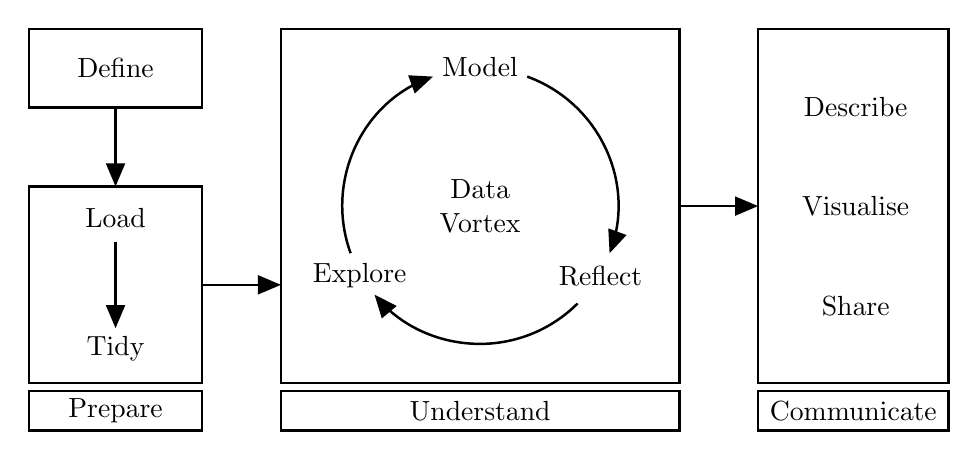
\begin{tikzpicture}[line width=.9pt]
% Block styles
\tikzstyle{set}=[inner sep=0pt, outer sep=0pt, draw=black, black, align=center, minimum width=2.2cm]
\tikzstyle{set2}=[inner sep=0pt, outer sep=0pt, draw=black, black, align=center, minimum width=2.2*2.3cm]
\tikzstyle{set3}=[inner sep=0pt, outer sep=0pt, draw=black, black, align=center, minimum width=2.2*1.1cm]
% Col 1
\node[set, minimum height=1cm] (A) {Define};
\node[set, minimum height=2.5cm, below=1cm of A] (B) {Load\\[12mm]Tidy};
\node[set, minimum height=.5cm, below=1mm of B] (C) {Prepare};
% Col 2
\node[set2, minimum height=4.5cm, anchor=north west] (A1) at ([xshift=1cm]A.north east) {};
\node[set2, minimum height=.5cm, below=1mm of A1] (B1) {Understand};
% Col 3
\node[set3, minimum height=4.5cm, anchor=north west] (A2) at ([xshift=1cm]A1.north east) {};
\node[set3, minimum height=.5cm, below=1mm of A2] (B2) {Communicate};
\node[align=center] at (9.4, -1.75) {Describe\\\\\\Visualise\\\\\\Share};
% Invisible circle including text
\node[circle, minimum size=3.5cm, align=center] (T) at (A1.center) {Data\\Vortex};
\node (exp) at (T.90+120) {Explore};
\node (ref) at (T.90-120) {Reflect};
\node (mod) at (T.90) {Model};
% Arrows
\draw[-triangle 45] (A)--(B);
\draw[-triangle 45, shorten <=7mm, shorten >=7mm] (B.90)--(B.-90);
\coordinate (p1) at (A1.west);
\draw[-triangle 45] (B)--(B-|p1);
\coordinate (p2) at (A2.west);
\draw[-triangle 45] (A1)--(A1-|p2);
\coordinate (p3) at (T.center);
\draw[triangle 45-] (p3)+(-20:3.5/2) arc (-20:70:3.5/2);
\draw[triangle 45-] (p3)+(110:3.5/2) arc (110:200:3.5/2);
\draw[triangle 45-] (p3)+(220:3.5/2) arc (220:315:3.5/2);
\end{tikzpicture}
\end{document}
